
\documentclass[10pt]{article}

\usepackage[a4paper,margin=0.65in]{geometry}
\usepackage{amsmath,amssymb}
\usepackage{graphicx}
\usepackage{booktabs}
\usepackage{array}
\usepackage{float}
\usepackage{hyperref}
\usepackage{enumitem}
\usepackage{xcolor}
\usepackage{tikz}
\usetikzlibrary{positioning,arrows.meta,shapes.geometric,fit,calc}

\setlist{nosep,leftmargin=*}
\renewcommand{\arraystretch}{1.2}
\setlength{\parindent}{0pt}
\setlength{\parskip}{2pt}

\tikzset{
layer/.style={
draw,
rounded corners,
minimum width=1.7cm,
minimum height=0.65cm,
align=center,
fill=blue!10,
font=\scriptsize
},
smalllayer/.style={
draw,
rounded corners,
minimum width=1.35cm,
minimum height=0.58cm,
align=center,
fill=green!10,
font=\scriptsize
},
arrow/.style={
-{Latex[length=2mm]},
thin
}
}

\begin{document}

%%%%%%%%%%%%%%%%%%%%%%%%%%%%%%%%%%%%%%%%%%%%%%%%%%%%%%%%%%%%
% TITLE
%%%%%%%%%%%%%%%%%%%%%%%%%%%%%%%%%%%%%%%%%%%%%%%%%%%%%%%%%%%%

\begin{center}

{\large\textbf{Shiv Nadar University Chennai}}

\vspace{2mm}

{\normalsize\textbf{CS3807 -- Deep Learning Laboratory}}

\vspace{2mm}

{\large\textbf{Experiment 7}}

\vspace{1mm}

{\normalsize\textbf{End-to-End Study of Autoencoders, Convolutional}}

{\normalsize\textbf{Autoencoders, Denoising Autoencoders and Variational Autoencoders}}

\end{center}

\vspace{3mm}

\begin{tabular}{|p{3.4cm}|p{9.0cm}|p{1.4cm}|}
\hline
Degree \& Branch &
B.Tech Artificial Intelligence \& Data Science &
Semester V\\
\hline
Subject Code \& Name &
CS3807 -- Deep Learning Laboratory &
AY: 2026--27\\
\hline
\end{tabular}

%%%%%%%%%%%%%%%%%%%%%%%%%%%%%%%%%%%%%%%%%%%%%%%%%%%%%%%%%%%%
\section*{1. Objective}

The objective of this experiment is to develop an end-to-end understanding of
autoencoders and their variants for image representation, reconstruction,
denoising and generative modeling.

The experiment begins with a fully connected autoencoder, progresses to a
Convolutional Autoencoder (CAE), introduces image corruption for denoising,
and finally develops a Variational Autoencoder (VAE). Students will visualize
the learned latent representation, compare reconstruction quality using
quantitative and qualitative measures, and explore the generative capability
of the VAE.

The same image dataset and a controlled experimental protocol should be used
throughout the experiment wherever possible.

%%%%%%%%%%%%%%%%%%%%%%%%%%%%%%%%%%%%%%%%%%%%%%%%%%%%%%%%%%%%
\section*{2. Learning Outcomes}

After completing this experiment, students will be able to:

\begin{itemize}
\item explain the encoder--latent--decoder structure of an autoencoder;
\item prepare image data for reconstruction-based learning;
\item implement a fully connected autoencoder;
\item implement a Convolutional Autoencoder for image reconstruction;
\item introduce controlled noise and build a denoising autoencoder;
\item evaluate reconstruction using MSE, MAE and SSIM;
\item visualize and interpret latent representations;
\item explain the probabilistic latent representation of a VAE;
\item implement the reparameterization trick;
\item calculate and interpret reconstruction and KL-divergence losses;
\item generate new images by sampling from a learned latent space; and
\item compare deterministic and variational latent representations.
\end{itemize}

%%%%%%%%%%%%%%%%%%%%%%%%%%%%%%%%%%%%%%%%%%%%%%%%%%%%%%%%%%%%
\section*{3. Dataset and Experimental Setup}

\textbf{Dataset: MNIST Handwritten Digit Dataset}

MNIST contains grayscale images of handwritten digits from 0 to 9. Each image
has spatial dimensions

\[
28\times28\times1.
\]

The dataset is particularly suitable for this experiment because the images
are small, the classes have visually meaningful structure, and the same image
format can be directly supplied to fully connected, convolutional and
variational autoencoders.

The dataset can be loaded directly using Keras/TensorFlow:

\url{https://www.tensorflow.org/api_docs/python/tf/keras/datasets/mnist}

\textbf{Recommended laboratory subset:}

Use 10,000 training images and 2,000 test images for the main laboratory
execution. The full MNIST dataset may be used if computational resources
permit.

The labels are not required as reconstruction targets. The original image is
the target:

\[
\boxed{x\rightarrow \text{Encoder}\rightarrow z
\rightarrow\text{Decoder}\rightarrow\hat{x}}
\]

where $x$ is the input image and $\hat{x}$ is its reconstruction.

%%%%%%%%%%%%%%%%%%%%%%%%%%%%%%%%%%%%%%%%%%%%%%%%%%%%%%%%%%%%
\section*{4. Expected Input and Output}

\subsection*{Expected Input}

Each input image has shape

\[
28\times28\times1.
\]

For a batch of 32 images:

\[
X\in\mathbb{R}^{32\times28\times28\times1}.
\]

Pixel values should be converted from

\[
[0,255]\rightarrow[0,1].
\]

For a fully connected autoencoder, the image may be flattened:

\[
28\times28=784.
\]

Therefore,

\[
x\in\mathbb{R}^{784}.
\]

For a convolutional autoencoder, retain the spatial structure:

\[
x\in\mathbb{R}^{28\times28\times1}.
\]

\subsection*{Expected Output}

The primary output is a reconstructed image:

\[
\hat{x}\in\mathbb{R}^{28\times28\times1}.
\]

Students must display:

\begin{verbatim}
Original image
Reconstructed image
Reconstruction error
\end{verbatim}

For the denoising model, display:

\begin{verbatim}
Original clean image
Noisy image
Denoised reconstruction
\end{verbatim}

For the VAE, display newly generated samples obtained by sampling from the
latent distribution.

%%%%%%%%%%%%%%%%%%%%%%%%%%%%%%%%%%%%%%%%%%%%%%%%%%%%%%%%%%%%
\section*{5. Overall Experimental Pipeline}

The complete experiment follows:

\begin{center}
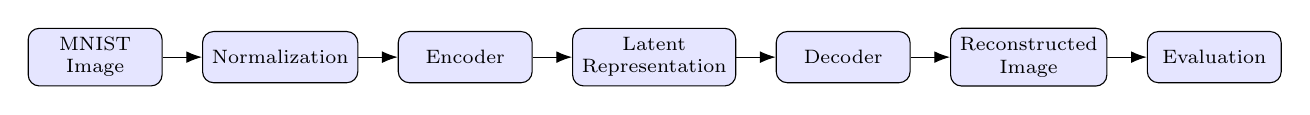
\begin{tikzpicture}[node distance=5mm]
\node[layer](a){MNIST\\Image};
\node[layer,right=of a](b){Normalization};
\node[layer,right=of b](c){Encoder};
\node[layer,right=of c](d){Latent\\Representation};
\node[layer,right=of d](e){Decoder};
\node[layer,right=of e](f){Reconstructed\\Image};
\node[layer,right=of f](g){Evaluation};

\foreach \x/\y in {a/b,b/c,c/d,d/e,e/f,f/g}
\draw[arrow](\x)--(\y);
\end{tikzpicture}
\end{center}

The experiment consists of four related studies:

\begin{enumerate}
\item Fully Connected Autoencoder
\item Convolutional Autoencoder
\item Denoising Convolutional Autoencoder
\item Variational Autoencoder
\end{enumerate}

%%%%%%%%%%%%%%%%%%%%%%%%%%%%%%%%%%%%%%%%%%%%%%%%%%%%%%%%%%%%
\section*{6. Exploring Autoencoders}

An autoencoder learns to reproduce its input at the output.

The encoder maps the input to a lower-dimensional representation:

\[
z=f_{\theta}(x),
\]

and the decoder reconstructs the input:

\[
\hat{x}=g_{\phi}(z).
\]

The training objective is to minimize reconstruction error:

\[
\mathcal{L}_{rec}
=
\frac{1}{N}\sum_{i=1}^{N}
\|x_i-\hat{x}_i\|^2.
\]

\begin{center}
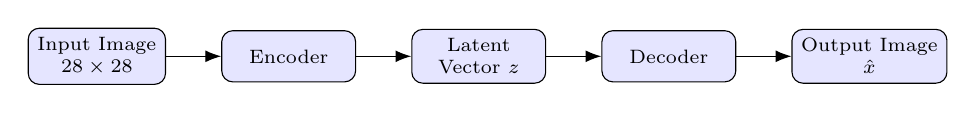
\begin{tikzpicture}[node distance=7mm]
\node[layer](a){Input Image\\$28\times28$};
\node[layer,right=of a](b){Encoder};
\node[layer,right=of b](c){Latent\\Vector $z$};
\node[layer,right=of c](d){Decoder};
\node[layer,right=of d](e){Output Image\\$\hat{x}$};

\foreach \x/\y in {a/b,b/c,c/d,d/e}
\draw[arrow](\x)--(\y);
\end{tikzpicture}
\end{center}

The latent vector is a compressed representation of the input.

%%%%%%%%%%%%%%%%%%%%%%%%%%%%%%%%%%%%%%%%%%%%%%%%%%%%%%%%%%%%
\section*{7. Fully Connected Autoencoder}

Flatten each image from

\[
28\times28=784
\]

to a vector of length 784.

Use the following architecture:

\begin{center}
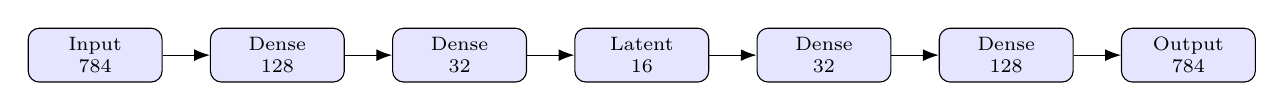
\begin{tikzpicture}[node distance=6mm]
\node[layer](a){Input\\784};
\node[layer,right=of a](b){Dense\\128};
\node[layer,right=of b](c){Dense\\32};
\node[layer,right=of c](d){Latent\\16};
\node[layer,right=of d](e){Dense\\32};
\node[layer,right=of e](f){Dense\\128};
\node[layer,right=of f](g){Output\\784};

\foreach \x/\y in {a/b,b/c,c/d,d/e,e/f,f/g}
\draw[arrow](\x)--(\y);
\end{tikzpicture}
\end{center}

Use ReLU activation in hidden layers and sigmoid activation in the output
layer.

\textbf{Suggested configuration:}

\begin{center}
\begin{tabular}{|l|l|}
\hline
Parameter & Value\\
\hline
Latent dimension & 16\\
Optimizer & Adam\\
Learning rate & $10^{-3}$\\
Batch size & 128\\
Epochs & 20\\
Loss & Binary Cross-Entropy\\
\hline
\end{tabular}
\end{center}

%%%%%%%%%%%%%%%%%%%%%%%%%%%%%%%%%%%%%%%%%%%%%%%%%%%%%%%%%%%%
\section*{8. Required Analysis of the Basic Autoencoder}

\textbf{Plot 1: Original versus Reconstructed Images}

Display at least 10 test images in a grid.

For every image, show:

\[
\text{Original}\quad|\quad\text{Reconstruction}.
\]

Students must comment on:

\begin{itemize}
\item preservation of digit shape;
\item loss of fine details;
\item blurred regions;
\item differences between easy and difficult samples.
\end{itemize}

\begin{figure}[H]
\centering
\includegraphics[width=0.9\linewidth]{plot1_original_vs_reconstructed.eps}
\caption{Original versus Reconstructed Images}
\label{fig:originalvsreconstructed}
\end{figure}

The plot shows that the autoencoder reconstructs the basic shapes of most digits, but some fine details appear slightly blurred.
This happens because the 16-dimensional latent space compresses the original image, so the model retains important features while losing minor details.

\textbf{Plot 2: Training and Validation Reconstruction Loss}

\begin{itemize}
\item X-axis: Epoch
\item Y-axis: Reconstruction loss
\item Curves: Training loss and validation loss
\end{itemize}

\textbf{Required inference:} Determine whether the model converges and whether
there is evidence of overfitting.

\begin{figure}[H]
\centering
\includegraphics[width=0.9\linewidth]{plot2_fcae_training_validation_loss.eps}
\caption{Training and Validation Reconstruction Loss}
\label{fig:trainingvsvalidation}
\end{figure}

Both training and validation losses decrease and gradually stabilize, showing that the autoencoder is learning and converging.
Since the two curves remain relatively close, there is no strong sign of overfitting.

%%%%%%%%%%%%%%%%%%%%%%%%%%%%%%%%%%%%%%%%%%%%%%%%%%%%%%%%%%%%
\section*{9. Reconstruction Metrics}

Students must calculate the following metrics on the test set.

\subsection*{Mean Squared Error}

\[
MSE=
\frac{1}{N}
\sum_{i=1}^{N}
(x_i-\hat{x}_i)^2.
\]

\subsection*{Mean Absolute Error}

\[
MAE=
\frac{1}{N}
\sum_{i=1}^{N}
|x_i-\hat{x}_i|.
\]

\subsection*{Structural Similarity}

Calculate SSIM between the original and reconstructed images.

The implementation may use:

\url{https://scikit-image.org/docs/stable/api/skimage.metrics.html}

Report:

\begin{center}
\begin{tabular}{|l|c|}
\hline
Metric & Value\\
\hline
Test MSE & 0.020302\\
Test MAE & 0.055554\\
Mean SSIM & 0.767590
\\
\hline
\end{tabular}
\end{center}

%%%%%%%%%%%%%%%%%%%%%%%%%%%%%%%%%%%%%%%%%%%%%%%%%%%%%%%%%%%%
\section*{10. Convolutional Autoencoder}

A Convolutional Autoencoder preserves spatial structure and uses convolutional
operations in the encoder and upsampling/transposed convolution operations
in the decoder.

The conceptual architecture is:

\begin{center}
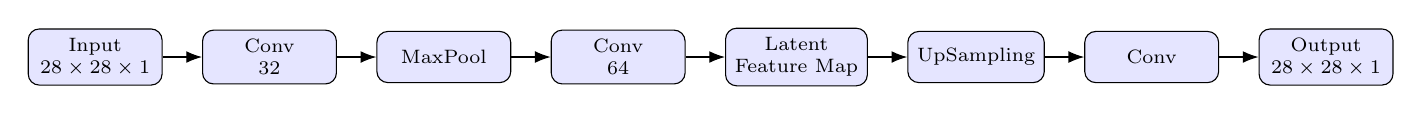
\begin{tikzpicture}[node distance=5mm]
\node[layer](a){Input\\$28\times28\times1$};
\node[layer,right=of a](b){Conv\\32};
\node[layer,right=of b](c){MaxPool};
\node[layer,right=of c](d){Conv\\64};
\node[layer,right=of d](e){Latent\\Feature Map};
\node[layer,right=of e](f){UpSampling};
\node[layer,right=of f](g){Conv};
\node[layer,right=of g](h){Output\\$28\times28\times1$};

\foreach \x/\y in {a/b,b/c,c/d,d/e,e/f,f/g,g/h}
\draw[arrow](\x)--(\y);
\end{tikzpicture}
\end{center}

A possible implementation is:

\begin{verbatim}
Input(28,28,1)
Conv2D(32, 3, activation='relu', padding='same')
MaxPooling2D(2, padding='same')
Conv2D(64, 3, activation='relu', padding='same')
MaxPooling2D(2, padding='same')
Conv2D(64, 3, activation='relu', padding='same')
UpSampling2D(2)
Conv2D(32, 3, activation='relu', padding='same')
UpSampling2D(2)
Conv2D(1, 3, activation='sigmoid', padding='same')
\end{verbatim}

The exact implementation may use Conv2DTranspose instead of UpSampling2D.

%%%%%%%%%%%%%%%%%%%%%%%%%%%%%%%%%%%%%%%%%%%%%%%%%%%%%%%%%%%%
\section*{11. Comparing Fully Connected and Convolutional Autoencoders}

Train both models using the same training and test images.

\begin{center}
\begin{tabular}{|l|c|c|c|c|}
\hline
Model & MSE & MAE & SSIM & Parameters\\
\hline
Fully Connected AE & 0.020302	 & 0.055554&0.767590 &211040\\
Convolutional AE &0.002598 &0.015472	 &0.972571	 &74497
\\
\hline
\end{tabular}
\end{center}

\textbf{Plot 3: Reconstruction Comparison}

Display:

\[
\text{Original}
\rightarrow
\text{FC-AE Reconstruction}
\rightarrow
\text{CAE Reconstruction}.
\]

\textbf{Required inference:}

Discuss how preserving spatial locality through convolution affects image
reconstruction.

\begin{figure}[H]
\centering
\includegraphics[width=0.9\linewidth]{plot3_fc_vs_conv_reconstruction.eps}
\caption{Reconstruction Comparison}
\label{fig:ReconstructionComparison}
\end{figure}

The convolutional autoencoder produces noticeably sharper reconstructions than the fully connected autoencoder.
This is because convolutions preserve local spatial information such as edges and shapes, resulting in much better reconstruction quality.

%%%%%%%%%%%%%%%%%%%%%%%%%%%%%%%%%%%%%%%%%%%%%%%%%%%%%%%%%%%%
\section*{12. Denoising Autoencoder}

A denoising autoencoder receives a corrupted image but is trained to
reconstruct the original clean image.

The training mapping is:

\[
\boxed{\tilde{x}\rightarrow\text{Encoder}\rightarrow z
\rightarrow\text{Decoder}\rightarrow\hat{x}}
\]

where $\tilde{x}$ is a noisy version of the clean image $x$.

\begin{center}
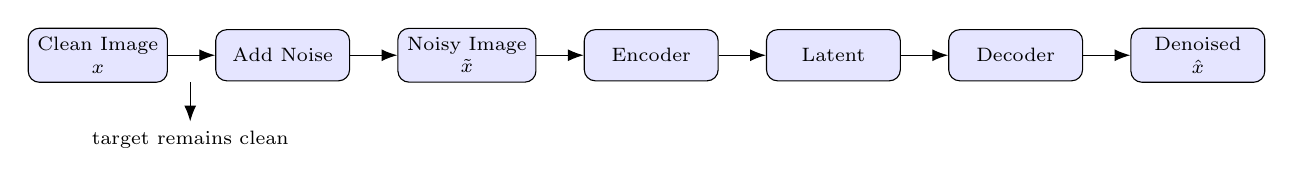
\begin{tikzpicture}[node distance=6mm]
\node[layer](a){Clean Image\\$x$};
\node[layer,right=of a](b){Add Noise};
\node[layer,right=of b](c){Noisy Image\\$\tilde{x}$};
\node[layer,right=of c](d){Encoder};
\node[layer,right=of d](e){Latent};
\node[layer,right=of e](f){Decoder};
\node[layer,right=of f](g){Denoised\\$\hat{x}$};

\foreach \x/\y in {a/b,b/c,c/d,d/e,e/f,f/g}
\draw[arrow](\x)--(\y);

\draw[arrow]($(a.south)!0.5!(b.south)$) -- ++(0,-5mm)
node[below,font=\scriptsize]{target remains clean};
\end{tikzpicture}
\end{center}

%%%%%%%%%%%%%%%%%%%%%%%%%%%%%%%%%%%%%%%%%%%%%%%%%%%%%%%%%%%%
\section*{13. Adding Image Noise}

Use at least two corruption types.

\subsection*{Gaussian Noise}

\[
\tilde{x}=x+n,
\qquad
n\sim\mathcal{N}(0,\sigma^2).
\]

Suggested standard deviations:

\[
\sigma\in\{0.1,0.2,0.3\}.
\]

Clip the resulting image to the range $[0,1]$.

\subsection*{Salt-and-Pepper Noise}

Randomly replace a small proportion of pixels with values close to 0 or 1.

Suggested corruption levels:

\[
p\in\{0.05,0.10,0.20\}.
\]

%%%%%%%%%%%%%%%%%%%%%%%%%%%%%%%%%%%%%%%%%%%%%%%%%%%%%%%%%%%%
\section*{14. Required Denoising Plots}

\textbf{Plot 4: Clean vs. Noisy vs. Denoised}

For at least 10 images, display:

\[
\text{Clean}\quad|\quad
\text{Noisy}\quad|\quad
\text{Denoised}.
\]

\begin{figure}[H]
\centering
\includegraphics[width=0.9\linewidth]{plot4_clean_noisy_denoised.eps}
\caption{Clean vs. Noisy vs. Denoised}
\label{fig:cleanvsnoisy}
\end{figure}

The plot shows that the denoising autoencoder removes much of the added noise while recovering the main structure of the original digit.
Although some small details may be lost, the model successfully learns to reconstruct clean images from corrupted inputs.

\textbf{Plot 5: Noise Level vs. Reconstruction Quality}

For each noise level, calculate:

\[
MSE,\quad MAE,\quad SSIM.
\]

\begin{figure}[H]
\centering
\includegraphics[width=0.9\linewidth]{plot5_noise_level_vs_quality.eps}
\caption{ Noise Level vs. Reconstruction Quality}
\label{fig:noisevsquality}
\end{figure}

As the noise level increases, MSE and MAE increase while SSIM decreases, indicating gradually poorer reconstruction quality.
Even at higher noise levels, the major digit structure is still recovered, showing that the denoising model is effective.

Report:

% \begin{center}
% \begin{tabular}{|c|c|c|c|}
% \hline
% Noise Level & MSE & MAE & SSIM\\
% \hline
% 0.1 & & &\\
% 0.2 & & &\\
% 0.3 & & &\\
% \hline
% \end{tabular}
% \end{center}

\begin{center}
\begin{tabular}{|c|c|c|c|}
\hline
Noise Level & MSE & MAE & SSIM\\
\hline
0.1 & 0.003579 & 0.017744 & 0.961529\\
0.2 & 0.004554 & 0.021068 & 0.948603\\
0.3 & 0.006917 & 0.028871 & 0.886132\\
\hline
\end{tabular}
\end{center}


\textbf{Required inference:}

Explain how increasing corruption affects reconstruction quality and identify
whether the denoising model is able to recover the major structure of the
original image.

%%%%%%%%%%%%%%%%%%%%%%%%%%%%%%%%%%%%%%%%%%%%%%%%%%%%%%%%%%%%
\section*{15. Variational Autoencoder}

A conventional autoencoder maps an input to a deterministic latent vector:

\[
z=f(x).
\]

A VAE instead learns a probability distribution:

\[
q_{\phi}(z|x)
=
\mathcal{N}
\left(
\mu(x),
\operatorname{diag}(\sigma^2(x))
\right).
\]

The encoder produces:

\[
\mu,\qquad \log\sigma^2.
\]

A latent vector is sampled using the reparameterization trick:

\[
z=\mu+\sigma\odot\epsilon,
\qquad
\epsilon\sim\mathcal{N}(0,I).
\]

\begin{center}
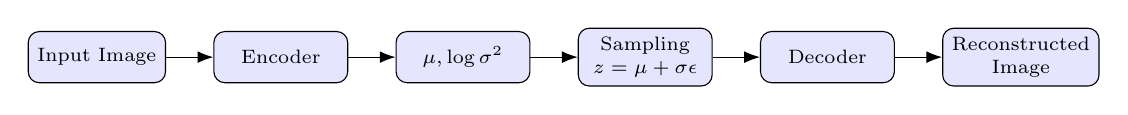
\begin{tikzpicture}[node distance=6mm]
\node[layer](a){Input Image};
\node[layer,right=of a](b){Encoder};
\node[layer,right=of b](c){$\mu,\log\sigma^2$};
\node[layer,right=of c](d){Sampling\\$z=\mu+\sigma\epsilon$};
\node[layer,right=of d](e){Decoder};
\node[layer,right=of e](f){Reconstructed\\Image};

\foreach \x/\y in {a/b,b/c,c/d,d/e,e/f}
\draw[arrow](\x)--(\y);
\end{tikzpicture}
\end{center}

%%%%%%%%%%%%%%%%%%%%%%%%%%%%%%%%%%%%%%%%%%%%%%%%%%%%%%%%%%%%
\section*{16. VAE Loss Function}

The VAE objective consists of two components.

\subsection*{Reconstruction Loss}

\[
\mathcal{L}_{rec}
=
-\mathbb{E}_{q_{\phi}(z|x)}
[\log p_{\theta}(x|z)].
\]

For normalized MNIST images, binary cross-entropy can be used.

\subsection*{KL Divergence}

\[
D_{KL}
\left(
q_{\phi}(z|x)\parallel p(z)
\right)
=
-\frac{1}{2}
\sum_j
\left(
1+\log\sigma_j^2-\mu_j^2-\sigma_j^2
\right).
\]

The total loss is

\[
\boxed{
\mathcal{L}_{VAE}
=
\mathcal{L}_{rec}
+
\mathcal{L}_{KL}
}
\]

where the prior is usually

\[
p(z)=\mathcal{N}(0,I).
\]

%%%%%%%%%%%%%%%%%%%%%%%%%%%%%%%%%%%%%%%%%%%%%%%%%%%%%%%%%%%%
\section*{17. VAE Implementation}

Use a small latent space so that it can be visualized.

Suggested latent dimension:

\[
z\in\mathbb{R}^{2}.
\]

The encoder should produce:

\[
\mu\in\mathbb{R}^{2},
\qquad
\log\sigma^2\in\mathbb{R}^{2}.
\]

The decoder maps

\[
z\rightarrow28\times28\times1.
\]

A compact architecture is:

\begin{center}
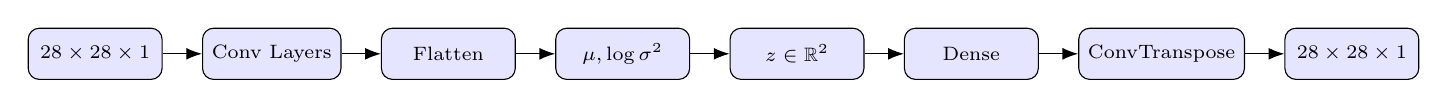
\begin{tikzpicture}[node distance=5mm]
\node[layer](a){$28\times28\times1$};
\node[layer,right=of a](b){Conv Layers};
\node[layer,right=of b](c){Flatten};
\node[layer,right=of c](d){$\mu,\log\sigma^2$};
\node[layer,right=of d](e){$z\in\mathbb{R}^2$};
\node[layer,right=of e](f){Dense};
\node[layer,right=of f](g){ConvTranspose};
\node[layer,right=of g](h){$28\times28\times1$};

\foreach \x/\y in {a/b,b/c,c/d,d/e,e/f,f/g,g/h}
\draw[arrow](\x)--(\y);
\end{tikzpicture}
\end{center}

%%%%%%%%%%%%%%%%%%%%%%%%%%%%%%%%%%%%%%%%%%%%%%%%%%%%%%%%%%%%
\section*{18. Exploring the VAE Latent Space}

Since the latent dimension is two, students can visualize the encoded test
images in a two-dimensional plane.

\textbf{Plot 6: VAE Latent Space}

\begin{itemize}
\item X-axis: $z_1$
\item Y-axis: $z_2$
\item Color/marker category: digit label
\end{itemize}

The labels are used only for visualization; they are not supplied to the VAE
during training.

\begin{figure}[H]
\centering
\includegraphics[width=0.9\linewidth]{plot6_vae_latent_space.eps}
\caption{VAE Latent Space}
\label{fig:latentspace}
\end{figure}

The latent-space plot shows that images of the same digit tend to form nearby regions, while some different digits overlap.
This indicates that the VAE learns meaningful but continuous representations rather than completely separated classes.

\textbf{Required inference:}

Students should describe whether samples belonging to the same digit occupy
similar regions and whether different digits overlap.

%%%%%%%%%%%%%%%%%%%%%%%%%%%%%%%%%%%%%%%%%%%%%%%%%%%%%%%%%%%%
\section*{19. Generating New Images with the VAE}

Sample points from

\[
z\sim\mathcal{N}(0,I).
\]

Pass the sampled latent vectors through the decoder.

\textbf{Plot 7: Randomly Generated Images}

Generate at least 25 images using randomly sampled latent vectors.

Display them in a grid.

Students should determine:

\begin{itemize}
\item whether the generated images resemble handwritten digits;
\item whether digit shapes are recognizable;
\item whether there is visible variation among generated samples; and
\item whether some samples are ambiguous or unrealistic.
\end{itemize}

\begin{figure}[H]
\centering
\includegraphics[width=0.9\linewidth]{plot7_vae_generated_images.eps}
\caption{Randomly Generated Images}
\label{fig:randomimages}
\end{figure}

The generated samples generally resemble handwritten digits, with visible variation between different samples.
Some images may be unclear or ambiguous because the VAE generates them by sampling from a learned probability distribution.

%%%%%%%%%%%%%%%%%%%%%%%%%%%%%%%%%%%%%%%%%%%%%%%%%%%%%%%%%%%%
\section*{20. Latent Space Interpolation}

Select two latent vectors:

\[
z_A,\qquad z_B.
\]

Construct

\[
z(\alpha)=(1-\alpha)z_A+\alpha z_B,
\qquad
\alpha\in[0,1].
\]

Use values such as:

\[
\alpha=
0,\;0.1,\;0.2,\ldots,1.
\]

Decode every interpolated vector.

\textbf{Plot 8: Latent Space Interpolation}

Display the decoded images in sequence.

\textbf{Required inference:}

Describe whether the decoded image changes smoothly as the latent vector moves
between two points.

\begin{figure}[H]
\centering
\includegraphics[width=0.9\linewidth]{plot8_latent_space_interpolation.eps}
\caption{Latent Space Interpolation}
\label{fig:latentspace}
\end{figure}
The generated digits change gradually as we move between two latent points, showing smooth transitions in the learned representation.
This suggests that the VAE has learned a continuous and meaningful latent space suitable for generating intermediate samples.

%%%%%%%%%%%%%%%%%%%%%%%%%%%%%%%%%%%%%%%%%%%%%%%%%%%%%%%%%%%%
\section*{21. Reconstruction Comparison Across Models}

Compare the three reconstruction-based models:


\begin{center}
\begin{tabular}{|l|c|c|c|c|}
\hline
Model & MSE & MAE & SSIM & Parameters\\
\hline
Fully Connected AE & 0.020302 & 0.055554 & 0.767590 & 211040\\
Convolutional AE & 0.002598 & 0.015472 & 0.972571 & 74497\\
Denoising CAE & 0.004540 & 0.021003 & 0.948701 & 74497\\
\hline
\end{tabular}
\end{center}


For the VAE, report its reconstruction loss separately because its total
objective also contains the KL-divergence term.

% \begin{center}
% \begin{tabular}{|l|c|}
% \hline
% VAE Metric & Value\\
% \hline
% Reconstruction Loss &\\
% KL Loss &\\
% Total Loss &\\
% Test MSE &\\
% Test MAE &\\
% Mean SSIM &\\
% \hline
% \end{tabular}
% \end{center}

\begin{center}
\begin{tabular}{|l|c|}
\hline
VAE Metric & Value\\
\hline
Reconstruction Loss & 155.023041\\
KL Loss & 5.586736\\
Total Loss & 160.609833\\
Test MSE & 0.046238\\
Test MAE & 0.105959\\
Mean SSIM & 0.493737\\
\hline
\end{tabular}
\end{center}


%%%%%%%%%%%%%%%%%%%%%%%%%%%%%%%%%%%%%%%%%%%%%%%%%%%%%%%%%%%%
\section*{22. Required Plots}

The final report must contain the following plots:

\begin{enumerate}
\item Original image versus reconstructed image.
\item Training and validation loss for the basic autoencoder.
\item Fully connected AE versus convolutional AE reconstruction.
\item Clean versus noisy versus denoised images.
\item Noise level versus MSE/MAE/SSIM.
\item VAE latent-space visualization.
\item Randomly generated VAE images.
\item Latent-space interpolation.
\item Training/validation reconstruction loss for the VAE.
\item Reconstruction-error distribution on the test set.
\end{enumerate}

For plots containing multiple quantitative measures, use separate figures or
clearly labeled axes rather than placing incompatible scales on one axis.

%%%%%%%%%%%%%%%%%%%%%%%%%%%%%%%%%%%%%%%%%%%%%%%%%%%%%%%%%%%%
\section*{23. Reconstruction Error Distribution}

Calculate the per-image reconstruction error:

\[
e_i=
\frac{1}{D}
\sum_{j=1}^{D}
(x_{ij}-\hat{x}_{ij})^2.
\]

\textbf{Plot 9: Distribution of Reconstruction Errors}

Plot a histogram of $e_i$ over the test set.

Students should identify:

\begin{itemize}
\item the typical reconstruction-error range;
\item whether the distribution is concentrated or spread out;
\item possible high-error samples; and
\item representative images corresponding to high reconstruction error.
\end{itemize}

\begin{figure}[H]
\centering
\includegraphics[width=0.9\linewidth]{plot9_vae_training_validation_loss.eps}
\caption{Distribution of Reconstruction Errors}
\label{fig:reconstructiondistribution}
\end{figure}
The training and validation reconstruction losses decrease during training and eventually become more stable, indicating that the VAE is learning to reconstruct the images.
The validation trend follows the training trend reasonably well, suggesting that the model generalizes without major overfitting.

%%%%%%%%%%%%%%%%%%%%%%%%%%%%%%%%%%%%%%%%%%%%%%%%%%%%%%%%%%%%
\section*{24. Required High-Error Image Analysis}

\begin{figure}[htbp]
    \centering
    \includegraphics[width=\textwidth,height=0.9\textheight,keepaspectratio]{plot_extra_section24_high_error_images-eps-converted-to.pdf}
    \caption{High-Error Image Analysis}
    \label{fig:large_figure}
\end{figure}


Select the five test images having the largest reconstruction errors.

Display:

\begin{center}
\begin{tabular}{|c|c|c|}
\hline
Sample & Original & Reconstruction\\
\hline
1 & &\\
2 & &\\
3 & &\\
4 & &\\
5 & &\\
\hline
\end{tabular}
\end{center}

% \begin{figure}[H]
% \centering
% \includegraphics[width=0.9\linewidth]{plot_extra_section24_high_error_images.eps}
% \caption{Distribution of Reconstruction Errors}
% \label{fig:reconstructiondistribution}
% \end{figure}






Students should provide a short explanation for why these images may be
difficult to reconstruct.

%%%%%%%%%%%%%%%%%%%%%%%%%%%%%%%%%%%%%%%%%%%%%%%%%%%%%%%%%%%%
\section*{25. Consolidated Results}



\begin{center}
\begin{tabular}{|l|c|c|c|c|c|}
\hline
Model & MSE & MAE & SSIM & Parameters & Time (s)\\
\hline
FC Autoencoder & 0.020302 & 0.055554 & 0.767590 & 211040 & 30.820551\\
Conv. Autoencoder & 0.002598 & 0.015472 & 0.972571 & 74497 & 20.536285\\
Denoising CAE & 0.004540 & 0.021003 & 0.948701 & 74497 & 18.845357\\
VAE & 0.046238 & 0.105959 & 0.493737 & 134165 & 33.472373\\
\hline
\end{tabular}
\end{center}


The values must be obtained from the student's own execution.

%%%%%%%%%%%%%%%%%%%%%%%%%%%%%%%%%%%%%%%%%%%%%%%%%%%%%%%%%%%%
\section*{26. Required Inferences}

For every major plot, students must write a short inference containing:

\begin{enumerate}
\item What does the plot show?
\item What trend is observed?
\item Why might the observed trend occur?
\item What conclusion can be drawn?
\end{enumerate}

The following inferences are mandatory:

\begin{itemize}
\item effect of latent dimension on reconstruction;
\item difference between fully connected and convolutional reconstruction;
\item effect of Gaussian noise level;
\item ability of the denoising autoencoder to recover image structure;
\item characteristics of the VAE latent distribution;
\item structure of the two-dimensional VAE latent space;
\item quality and diversity of generated samples;
\item smoothness of latent-space interpolation;
\item relationship between reconstruction error and visual quality; and
\item differences between deterministic and probabilistic latent representations.
\end{itemize}

\begin{itemize}

\item \textbf{Effect of latent dimension on reconstruction:} Increasing latent dimension reduces reconstruction error and improves image quality, but decreases compression. 

\item \textbf{Fully connected vs. convolutional reconstruction:} The convolutional autoencoder gives sharper and more accurate reconstructions by preserving spatial features better. 

\item \textbf{Effect of Gaussian noise level:} Increasing noise increases MSE and MAE while reducing SSIM, leading to poorer reconstruction quality. 

\item \textbf{Denoising autoencoder:} The denoising autoencoder removes noise effectively and recovers the main structure of the original digits.

\item \textbf{VAE latent distribution:} The VAE learns a continuous probabilistic latent distribution that supports sampling and generation of new images. 
\item \textbf{Two-dimensional VAE latent space:} Similar digits tend to cluster together, showing that the latent space captures meaningful image similarities. 

\item \textbf{Generated samples:} The generated images resemble handwritten digits and show variation, although some may appear blurred or unclear. 
\item \textbf{Latent-space interpolation:} The generated images change smoothly between latent points, indicating a continuous and meaningful latent space. 

\item \textbf{Reconstruction error and visual quality:} Lower reconstruction error generally corresponds to better visual similarity, while high-error images show larger differences. 

\item \textbf{Deterministic vs. probabilistic representations:} A basic autoencoder learns a fixed latent vector, whereas a VAE learns a probability distribution, enabling image generation. 

\end{itemize}

%%%%%%%%%%%%%%%%%%%%%%%%%%%%%%%%%%%%%%%%%%%%%%%%%%%%%%%%%%%%
\section*{27. Additional Latent-Dimension Study}

Repeat the basic autoencoder using:

\[
d_z\in\{2,8,16,32\}.
\]

Report:

\begin{center}
\begin{tabular}{|c|c|c|c|}
\hline
Latent Dimension & MSE & SSIM & Parameters\\
\hline
2 & 0.047069 & 0.474146 & 210130\\
8 & 0.030331 & 0.668648 & 210520\\
16 & 0.021557 & 0.755710 & 211040\\
32 & 0.019286 & 0.782389 & 212080\\
\hline
\end{tabular}
\end{center}


\begin{figure}[H]
\centering
\includegraphics[width=0.9\linewidth]{plot_extra_section27_latent_dim_vs_mse.eps}
\caption{Latent Dimension vs. MSE}
\label{fig:dimvsmse}
\end{figure}
As the latent dimension increases from 2 to 32, the reconstruction MSE consistently decreases, showing better preservation of information.
The improvement occurs because a larger latent space stores more features, although this reduces the amount of compression.

\textbf{Plot 10: Latent Dimension vs. Reconstruction MSE}

Students should explain the trade-off between compression and reconstruction
quality.

\begin{figure}[H]
\centering
\includegraphics[width=0.9\linewidth]{plot10_reconstruction_error_distribution.eps}
\caption{Latent Dimension vs. Reconstruction MSE}
\label{fig:reconstructionmse}
\end{figure}
Most test images have relatively low reconstruction errors, while only a smaller number show noticeably higher errors.
High-error images are likely harder to reconstruct because of unusual digit shapes, writing styles, or less common visual patterns.
%%%%%%%%%%%%%%%%%%%%%%%%%%%%%%%%%%%%%%%%%%%%%%%%%%%%%%%%%%%%
% \section*{28. Discussion Questions}

% \begin{enumerate}
% \item What is an autoencoder?
% \item What is the purpose of the encoder?
% \item What is the purpose of the decoder?
% \item What is a latent representation?
% \item Why is the latent representation usually smaller than the input?
% \item What happens when the latent dimension is too small?
% \item What happens when the latent dimension is increased?
% \item Why can a convolutional autoencoder preserve spatial information more effectively?
% \item Differentiate an autoencoder and a denoising autoencoder.
% \item Why is the clean image used as the target in denoising?
% \item What happens when the noise level is increased?
% \item Why are MSE, MAE and SSIM useful for image reconstruction?
% \item What is a Variational Autoencoder?
% \item How does a VAE differ from a conventional autoencoder?
% \item Why does a VAE learn a distribution instead of a single latent vector?
% \item What is the reparameterization trick?
% \item Why is $\epsilon$ sampled from a standard normal distribution?
% \item What is the role of KL divergence in the VAE loss?
% \item What is the prior distribution used in the VAE?
% \item Why is a two-dimensional latent space useful for visualization?
% \item What does latent-space interpolation demonstrate?
% \item Why can a VAE generate new images?
% \item Why might some VAE-generated images be unclear?
% \item What is the difference between reconstruction and generation?
% \item Why should test images remain unseen during training?
% \end{enumerate}


\section*{28. Discussion Questions and Answers}

\begin{enumerate}

\item \textbf{What is an autoencoder?}\\
An autoencoder is a neural network that learns to reconstruct its input.

\item \textbf{What is the purpose of the encoder?}\\
It converts the input into a compact latent representation.

\item \textbf{What is the purpose of the decoder?}\\
It reconstructs the original input from the latent representation.

\item \textbf{What is a latent representation?}\\
It is a compact representation of the important features of the input.

\item \textbf{Why is the latent representation usually smaller than the input?}\\
To force the model to learn the most important features.

\item \textbf{What happens when the latent dimension is too small?}\\
Important information may be lost, causing poor reconstruction.

\item \textbf{What happens when the latent dimension is increased?}\\
Reconstruction generally improves, but compression decreases.

\item \textbf{Why can a convolutional autoencoder preserve spatial information more effectively?}\\
Convolutions capture local spatial patterns such as edges and textures.

\item \textbf{Differentiate an autoencoder and a denoising autoencoder.}\\
An autoencoder reconstructs the input; a denoising autoencoder reconstructs clean data from noisy input.

\item \textbf{Why is the clean image used as the target in denoising?}\\
It teaches the model to remove noise.

\item \textbf{What happens when the noise level is increased?}\\
Reconstruction becomes more difficult and image quality may decrease.

\item \textbf{Why are MSE, MAE and SSIM useful for image reconstruction?}\\
They measure different aspects of reconstruction quality.

\item \textbf{What is a Variational Autoencoder?}\\
A VAE is an autoencoder that learns a probability distribution in latent space.

\item \textbf{How does a VAE differ from a conventional autoencoder?}\\
A VAE learns a latent distribution, while a conventional autoencoder learns fixed latent representations.

\item \textbf{Why does a VAE learn a distribution instead of a single latent vector?}\\
To enable smooth sampling and generation of new data.

\item \textbf{What is the reparameterization trick?}\\
It allows random sampling while keeping the process differentiable.

\item \textbf{Why is $\epsilon$ sampled from a standard normal distribution?}\\
It provides a simple and fixed source of randomness.

\item \textbf{What is the role of KL divergence in the VAE loss?}\\
It keeps the learned latent distribution close to the prior distribution.

\item \textbf{What is the prior distribution used in the VAE?}\\
Usually, a standard normal distribution $\mathcal{N}(0,I)$.

\item \textbf{Why is a two-dimensional latent space useful for visualization?}\\
It can be easily plotted and analyzed visually.

\item \textbf{What does latent-space interpolation demonstrate?}\\
It shows smooth transitions between learned representations.

\item \textbf{Why can a VAE generate new images?}\\
New latent samples can be decoded into images.

\item \textbf{Why might some VAE-generated images be unclear?}\\
The latent distribution and reconstruction process may produce blurred outputs.

\item \textbf{What is the difference between reconstruction and generation?}\\
Reconstruction reproduces an input, while generation creates new samples.

\item \textbf{Why should test images remain unseen during training?}\\
To fairly evaluate the model's ability to generalize.

\end{enumerate}


%%%%%%%%%%%%%%%%%%%%%%%%%%%%%%%%%%%%%%%%%%%%%%%%%%%%%%%%%%%%
\section*{29. Additional Exercises}

\begin{enumerate}
\item Train the convolutional autoencoder with latent dimensions of 4, 8, 16
and 32 and compare reconstruction quality.

\begin{figure}[H]
\centering
\includegraphics[width=0.9\linewidth]{ex1_latent_size_vs_mse.eps}
\caption{Convolutional Autoencoder with latent dimensions of 4, 8, 16
and 32}
\label{fig:dim}
\end{figure}
\item Compare Gaussian noise and salt-and-pepper noise using the same denoising
architecture.

\begin{figure}[H]
\centering
\includegraphics[width=0.9\linewidth]{ex2_gaussian_vs_saltpepper.eps}
\caption{Gaussian noise and salt-and-pepper noise}
\label{fig:reconstructionmse}
\end{figure}
\item Train the denoising autoencoder using two different noise levels and
compare SSIM.

\begin{figure}[H]
\centering
\includegraphics[width=0.9\linewidth]{ex3_noise_levels_ssim.eps}
\caption{Comparison of SSIM}
\label{fig:reconstructionmse}
\end{figure}
\item Replace the convolutional decoder with transposed convolutions and
compare the reconstructions.

\begin{figure}[H]
\centering
\includegraphics[width=0.9\linewidth]{ex4_upsampling_vs_transpose.eps}
\caption{Upsampling vs Conv2DTranspose Decoder}
\label{fig:reconstructionmse}
\end{figure}
\item Implement a VAE with latent dimension 2 and 8 and compare the latent
representations.
\item Investigate the effect of increasing the KL-loss contribution.
\item Generate a larger grid of VAE samples and discuss diversity.

\begin{figure}[H]
\centering
\includegraphics[width=0.9\linewidth]{ex7_larger_vae_sample_grid.eps}
\caption{Larger grid of VAE samples }
\label{fig:reconstructionmse}
\end{figure}
\item Select two digit regions in the latent space and perform interpolation.
\end{enumerate}

%%%%%%%%%%%%%%%%%%%%%%%%%%%%%%%%%%%%%%%%%%%%%%%%%%%%%%%%%%%%
\section*{30. Expected Outcome}

At the end of the experiment, students should be able to demonstrate the
complete image-representation and reconstruction pipeline:

\[
\boxed{
\text{Image}
\rightarrow
\text{Encoder}
\rightarrow
\text{Latent Representation}
\rightarrow
\text{Decoder}
\rightarrow
\text{Reconstructed Image}
}
\]

They should also demonstrate denoising:

\[
\boxed{
\text{Clean Image}
\rightarrow
\text{Noise}
\rightarrow
\text{Denoising Autoencoder}
\rightarrow
\text{Recovered Image}
}
\]

and variational generation:

\[
\boxed{
\text{Image}
\rightarrow
(\mu,\sigma)
\rightarrow
z
\rightarrow
\text{Decoder}
\rightarrow
\text{Generated/Reconstructed Image}
}
\]

The final report should contain both quantitative evaluation and visual
analysis. Numerical performance values must be obtained from the student's
own execution.

%%%%%%%%%%%%%%%%%%%%%%%%%%%%%%%%%%%%%%%%%%%%%%%%%%%%%%%%%%%%

\section*{30. Source Code}


The complete source code, datasets, generated plots, and report files for this experiment are available in the following GitHub repository:



\noindent\textbf{GitHub Repository:} \\
\url{https://github.com/VIKASNI-S/Deep-Learning-Lab/tree/main/Lab-6}\\

\section*{31. References}

\begin{enumerate}
\item Ian Goodfellow, Yoshua Bengio and Aaron Courville,
\emph{Deep Learning}, MIT Press, 2016.

\item Diederik P. Kingma and Max Welling,
``Auto-Encoding Variational Bayes,'' ICLR, 2014.

\item Pascal Vincent et al.,
``Stacked Denoising Autoencoders: Learning Useful Representations in a Deep
Network with a Local Denoising Criterion,'' Journal of Machine Learning
Research, 2010.

\item Yann LeCun, Corinna Cortes and Christopher J. C. Burges,
``MNIST Handwritten Digit Database.''

\item TensorFlow Documentation:
\url{https://www.tensorflow.org}

\item Keras Documentation:
\url{https://keras.io}

\item scikit-image Documentation:
\url{https://scikit-image.org}
\end{enumerate}

\end{document}
